\section{Descrição do Problema}

\subsection{Grafos e Redes Muiltimodais}

\frame
{
\frametitle{Definição de Grafo}
\begin{block}{Definição}
``Um grafo é uma representação abstrata de um conjunto de objetos, onde alguns pares de objetos estão conectados por ligações.
As os objetos são representados por abstrações matemáticas chamadas vértices, e as ligações que conectam alguns dos pares de vértices são chamadas de arestas.''
%TODO: ref wiki 
\end{block}
}

\frame
{
\frametitle{Exemplo de Grafo}
\begin{columns}[c]
\column{1.5in}
	\begin{exampleblock}{Exemplo}
		$G = (V,E)$ \\
		$ $ \\
		$V = \{1,2,3,4\}$ \\
		$ $ \\
		$E = \{e_1,e_2,e_3,e_4\}$ 
	\end{exampleblock}
\column{1.5in}
	\begin{figure}
		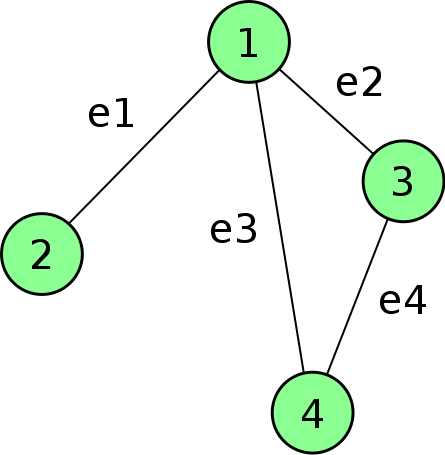
\includegraphics[width=\textwidth]{./imgs/grafo.png}
		\caption{Exemplo de grafo}
		%TODO: ref
		%\fonte{\citeonline{wikigrafo}}
	\end{figure}
\end{columns}
}

\frame
{
\frametitle{Redes Multimodais}
\begin{itemize}
	\item oi
\end{itemize}
}
